\subsection{Measurement routine and error bars}
\label{sec:exp:measroutine}

For each light-light characteristic
we vary the incident pump power $P$
and the temperature of the heat sink $\Ths$.
The varying heat sink temperature
is required to determine
the thermal resistance,
see section~\ref{sec:rth}.

The heat sink temperatures are partially set
in ascending and descending order, Fig.~\ref{img:temp_order}.
This allows us to save time,
since the heat reservoir
providing the temperature stabilized water
is inert.
On the other hand,
this routine also indicates
whether the results are consistent
or depend on the temperature cycle
they were measured in.
And last but not least,
this routine allows us
to see whether or not
the sample takes damage
as a result of the elevated temperature;
a property vital for real world applications.

\begin{figure}
\centering
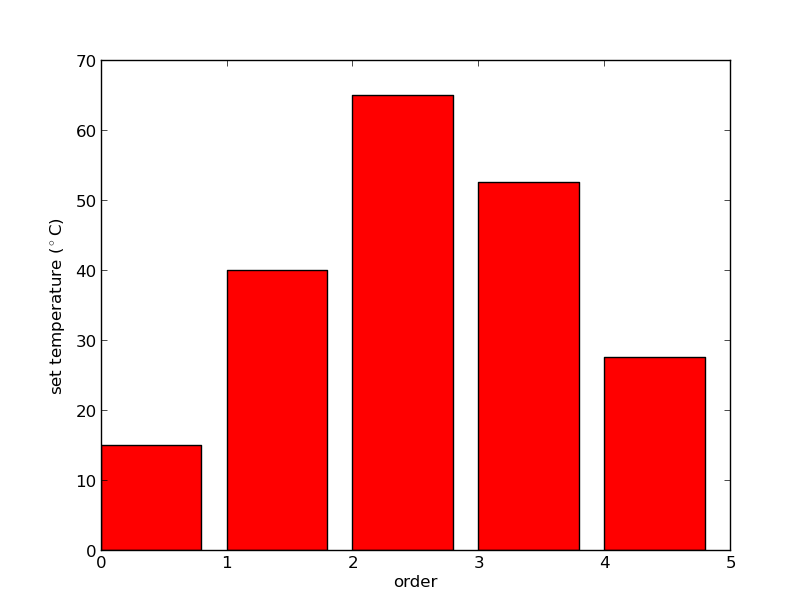
\includegraphics[width=6cm]{img/temp_order.png}
\caption{An example for the temperature order.
Some of the temperatures
are set
while heating up,
the rest while cooling down.
The objective is to save time,
to have a consistency check,
and to see whether the sample
shows fatigue after heating it up.}
\label{img:temp_order}
\end{figure}

At each heat sink temperature
we irradiate the sample
with different pump powers.
Each pump is repeated $N$ times over all.
The pump order is selected at random,
as illustrated in Fig.~\ref{img:random_sampling}.
Thanks to the random sampling
the measurement results
are detached from the lab environment --
most notably time-independent.
The heat sink cannot control its temperature
with absolute precision.
Figure~\ref{img:random_sampling_heatsink}
illustrates this issue:
It shows
the actually present heat sink temperature
for six set temperatures.
In the left column
the temperatures are plotted
in chronological order.
We can identify,
the temperature drifts.
The right column shows the same temperatures,
but corresponding to the set pump.
The repeated measurements
see a spread of different temperatures
but the temporal drifts can not be resolved.

In contrast,
Fig.~\ref{img:random_sampling_ramp_heatsink}
shows the heat sink temperature
during a measurement without the random pump selection.
In this case, clearly,
we cannot talk about a single heat sink temperature
for all the pump settings
for this specific set heat sink temperature.
The resulting measurements are highly repeatable,
but only given the same pump order.
This pseudo-stability
we exploit
during the calibration process
of the different beam samplers
and detectors:
During the calibration
we don't care about reproducibility
but solely about the repeatability
of two consecutive measurements.

\begin{figure}
\centering
\subfigure{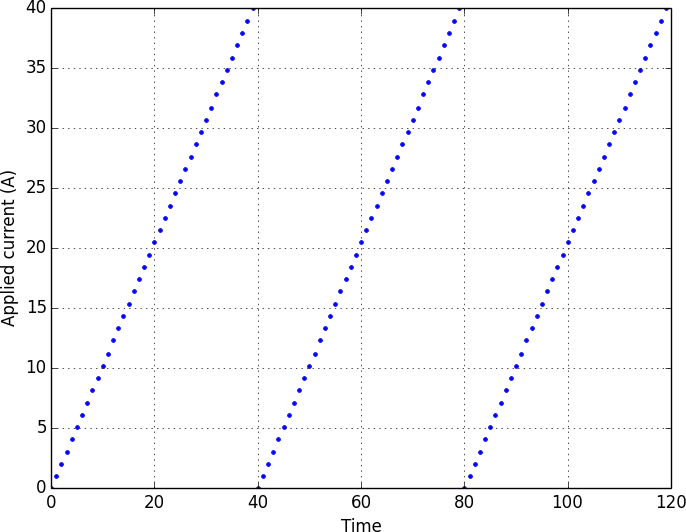
\includegraphics[width=7cm]{img/random_sampling_ramp.png}}
\subfigure{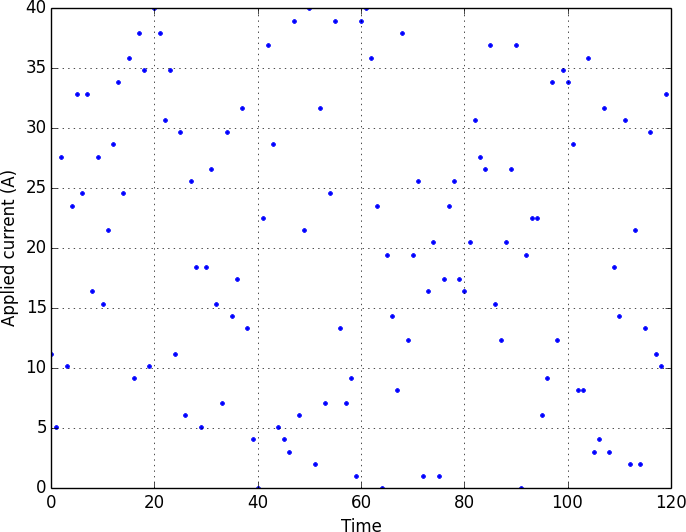
\includegraphics[width=7cm]{img/random_sampling_random.png}}
\caption{Two examples to apply various pump settings, with a repetition rate of 3.
Left: A ramp. Right: Random sampling.}
\label{img:random_sampling}
\end{figure}

\begin{figure}
\centering
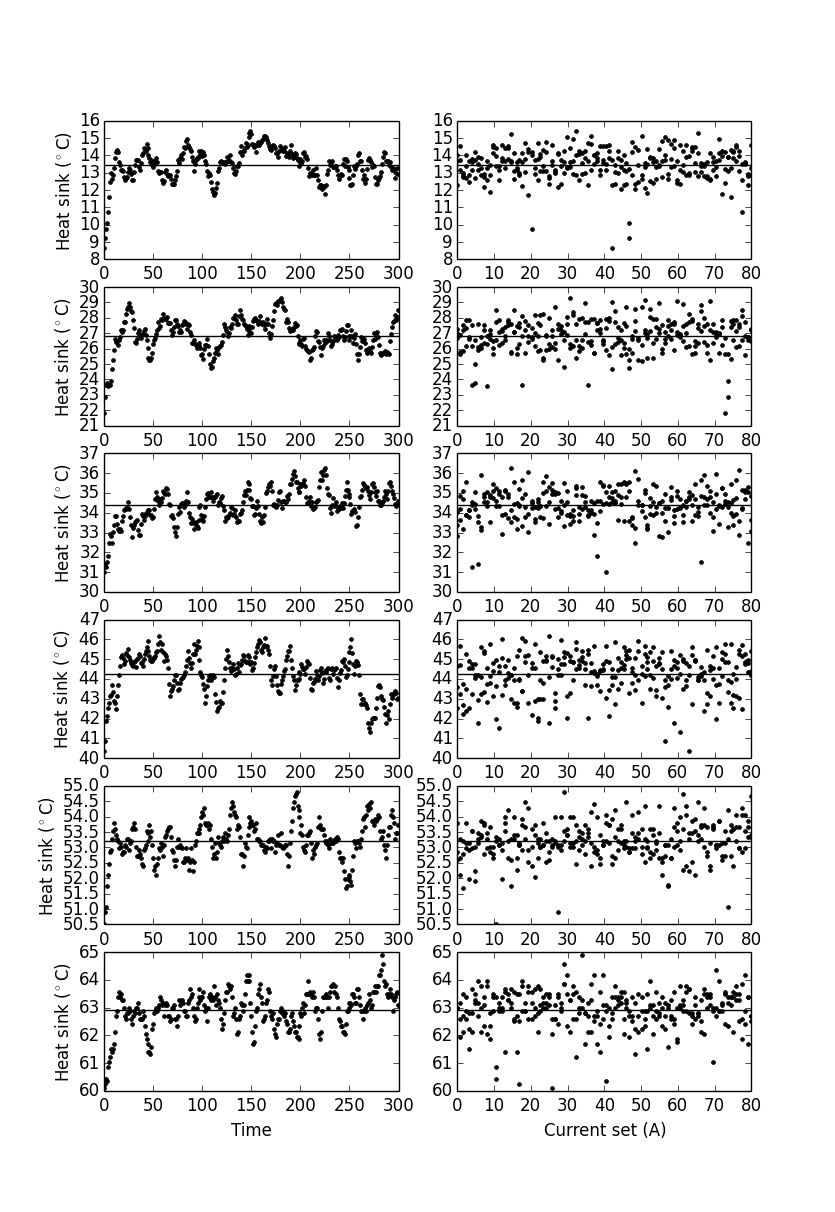
\includegraphics[width=15cm]{img/random_sampling_heatsink.png}
\caption{The heat sink temperature fluctuates over time (left).
Thanks to the random sampling addressed in Fig.~\ref{img:random_sampling}
the measurements don't see these drifts (right).}
\label{img:random_sampling_heatsink}
\end{figure}

\begin{figure}
\centering
\subfigure{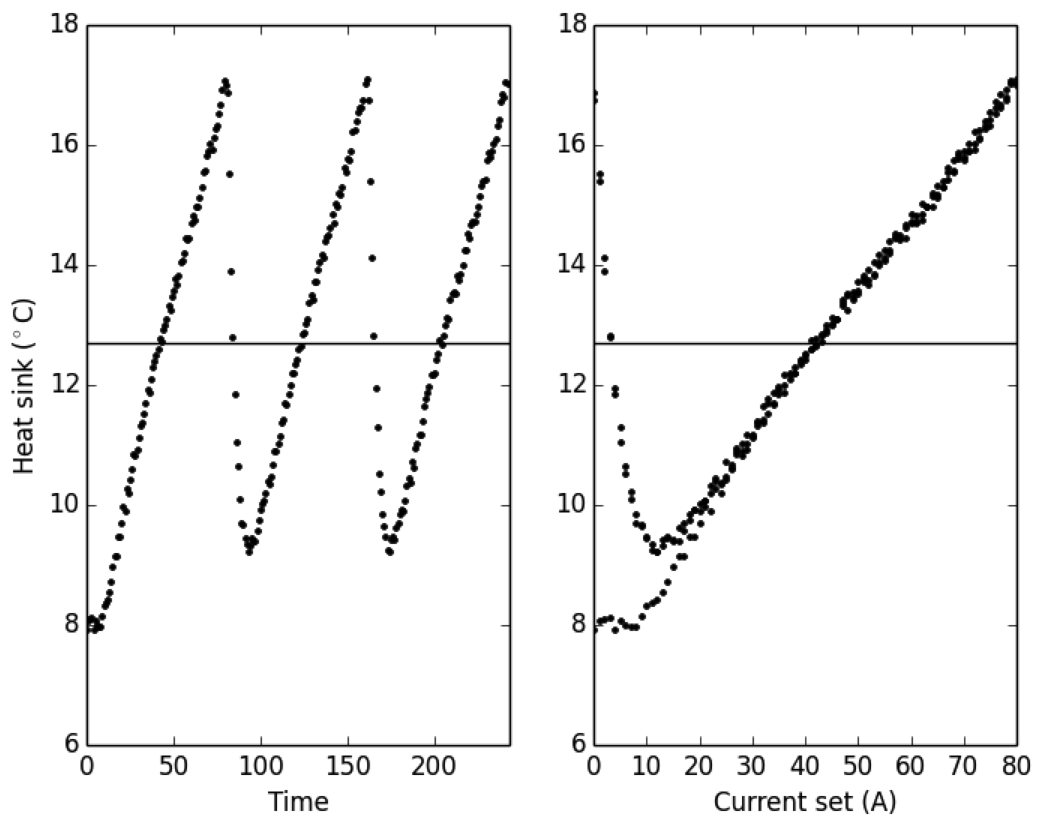
\includegraphics[width=7cm]{img/random_sampling_ramp_heatsink.png}}
\subfigure{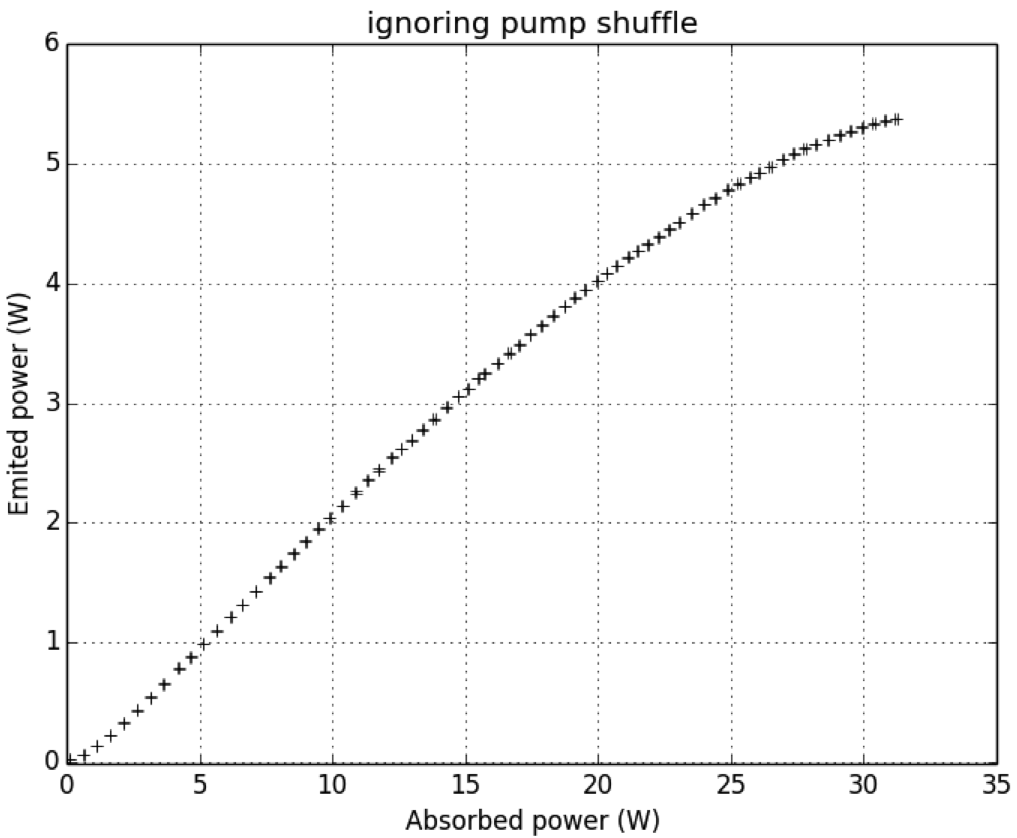
\includegraphics[width=7cm]{img/random_sampling_ramp_noisfreeLL.png}}
\caption{In contrast to Fig.~\ref{img:random_sampling_heatsink},
when we ignore the random pump sampling
highlighted in Fig.~\ref{img:random_sampling},
the temperature seen by the single pump settings
differ strongly from the average heat sink temperature
(left).
The resulting LL-characteristic
has very little noise on its data points
(right).
But these small error bars dismiss the fact
that the underlying points were measured
under very different conditions;
eroding the significance
of this low noise.}
\label{img:random_sampling_ramp_heatsink}
\end{figure}

The power meter average each measurement point
over 200 samples,
of which each one sample
takes approx. 3 ms \cite{ThorlabsPM}.

As mentioned already,
we repeated the measurement of each pump setting
$N$ times.
With this repetition we obtain a measure
for how well we know
the underlying true value.
We are hence interested in
the mean of these single measurements and
the resulting unbiased standard error \cite{Barlow}
\begin{equation}
\Delta x = \sqrt{ \frac{1}{N(N-1)}
	\sum\limits_{i=1}^N (x_i - 
		\frac{1}{N} \sum\limits_{i=1}^N x_i )^2 }.
\label{eq:sterr}
\end{equation}

For the uncertainties attached to
quantities obtained through fits,
I use a so-called
Jackknife \cite{Efron1983} approach:
In a nutshell,
this method allows to estimate
the influence of the single measurement points
on the fit parameters
without working through
the covariance matrix of the fit.
The resulting error value
is directly related with the
unbiased standard error (\ref{eq:sterr}),
used for the rest of the report.